%%%%%%%%%%%%%%%%%%%%%%%%%%%%%%%%%%%%%%%%%%%%%%%%%%%%%%%%%%%%%%%%%%%%%%%%
\chapter{Introduction}
%%%%%%%%%%%%%%%%%%%%%%%%%%%%%%%%%%%%%%%%%%%%%%%%%%%%%%%%%%%%%%%%%%%%%%%%

\begin{center}
    \begin{minipage}{0.5\textwidth}
        \begin{small}
            In which the reasons for doing this Ph.D. are laid bare for the whole world to see and we encounter some answers to questions in which, frankly, only an extremely small number of people were interested in the first place.
        \end{small}
    \end{minipage}
    \vspace{0.5cm}
\end{center}

\section{The BASNUM Project}

This thesis is part of the ANR BASNUM project (ANR-18-CE38-0003), which had as its main objective to digitize the \enquote{\emph{Dictionnaire Universel}} (DU) of Antoine Furetière, in its 1701 version reviewed and corrected by Basnage from Beauval \citep{furetiere-1701-dictionnaire}, and to analyze it with digital tools, in order to reveal the importance of this work for the evolution of science and mentalities in the 18\textsuperscript{th} century. The project also aimed to contribute to the current movement to design innovative methods for digitizing, encoding and analyzing texts.

From a purely computational point of view, the BASNUM project intended to carry out two types of tasks:
\begin{enumerate}
    \item a first structuring task where the macrostructure of the dictionary would be annotated,
    \item a second enrichment task which consisted in carrying out a wide range of tasks of information extraction, annotation of the dictionary microstructure and even normalization and modernization of the text.
\end{enumerate}

The first task of automatically structuring dictionaries had been already partially covered by the work of \citet{khemakhem-etal-2017-automatic,khemakhem-etal-2018-enhancing} who developed \emph{GROBID-dictionaries}, a submodule of \emph{GROBID}\footnote{Machine learning library to extract, analyze and restructure raw documents such as PDFs into structured and TEI-encoded documents.} \citep{lopez-etal-2018-grobid} implementing a Java machine learning library for structuring digitized lexical resources in TEI \emph{TEI} format \citep{tei-2018-guidelines}, to enable analysis, extraction and structuring of textual information in such resources. \emph{GROBID-dictionaries} had already obtained promising results and performances \citep{khemakhem-2020-standard}, so much so that it was used to make a first annotation of the \emph{Dictionnaire Universel} macrostructure.

Given the work done by \citet{khemakhem-2020-standard}, we decided to concentrate on the second task of enriching the dictionaries, which at the time remained quite general and abstract, in particular in contrast to the first task of structuring. To approach this task, we had two options: either we develop multiple models and annotation systems dedicated to each of the subtasks involved in this \emph{enrichment} and solely targeting the \emph{Dictionnaire Universel}, or we developed a single generic annotation model capable of addressing all enrichment subtasks and capable of handling not only the \emph{Dictionnaire Universel}, but also other texts and resources from the modern period.\footnote{Between the 16th and 18th century.}

Given the nature of the enrichment task and the fact that new neural language models able to transfer knowledge between different tasks in natural language processing (NLP) had just been published at the beginning of this thesis \cite{peters-etal-2018-deep,devlin-etal-2019-bert}, we decided to focus on the second option and, accordingly, to develop a single general model that we hoped would be able to be used for all these enrichment tasks and for any type of document in Modern or Contemporary French.

By choosing this approach, we also wanted to approach in an indirect way the first task of automatic structuring, this is because we believed that it was possible to improve the first results of \emph{GROBID}-dictionaries by using new neural models. Indeed, \emph{GROBID}-dictionaries relied on CRF models (Conditional Random Fields) \cite{lafferty-etal-2001-conditional} which were widely used for token labeling and classification, but that had been superseded by these neural models in recent years \citep{lample-etal-2016-neural,devlin-etal-2019-bert}. Furthermore, we knew that the developers of \emph{GROBID} had started working with some of these neural models by writing \emph{DeLFT}, a library for text processing, covering token labeling and classification. This library reimplements the latest machine learning models in NLP \citep{lopez-etal-2018-delft} and aims to improve \emph{GROBID}'s pipelines. It is tools and ideas like those contained in \emph{DeLFT} that could be applied to \emph{GROBID}-Dictionaries to significantly improve and expand its capabilities for the benefit of the \emph{BASNUM} project, especially in addition to resources that we had decided to develop.


Having chosen to develop these new models for French, such as \emph{ELMo} \citep{peters-etal-2018-deep} or \emph{BERT} \cite{devlin-etal-2019-bert}, we had to start by building and collecting our own corpus for the pre-training of these architectures, since the contemporary French corpora freely available at the time, such as Wikipedia or frWAC \citep{baroni-etal-2009-the}, were not considered to be large enough for this \citep{liu-etal-2019-roberta}.

Our plan then was to develop a pre-training corpus for Contemporary French, then to pre-train a language model for Contemporary French and finally to use the knowledge transfer capabilities of these architectures to adapt it to Early Modern French, in case we were unable to find enough textual resources to directly pre-train such a language model for Early Modern French. During this thesis, we also wanted to investigate the question of the minimum amount of resources required to successfully pre-train such models, an amount which, at the time, was considered higher than what was available for historical languages \citep{peters-etal-2018-deep,liu-etal-2019-roberta}.

%%%%%%%%%%%%%%%%%%%%%%%%%%%%%%%%%%%%%%%%%%%%%%%%%%%%%%%%%%%%%%%%%%%%%%%%
\section{Transfer Learning in NLP}
%%%%%%%%%%%%%%%%%%%%%%%%%%%%%%%%%%%%%%%%%%%%%%%%%%%%%%%%%%%%%%%%%%%%%%%%

In recent years neural methods for Natural Language Processing (NLP) have consistently and repeatedly improved the state-of-the-art in a wide variety of NLP tasks such as parsing, PoS-tagging, named entity recognition, machine translation, text classification and reading comprehension among others. Probably the main contributing factor in this steady improvement for NLP models is the raise in usage of \emph{transfer learning} techniques in the field. These methods normally consist of taking a pre-trained model and reusing it, with little to no retraining, to solve a different task from the original one it was intended to solve; in other words, one \emph{transfers} the \emph{knowledge} from one task to another.

Most of the transfer learning done in NLP nowadays is done in an unsupervised manner, that is, it normally consists of a  \emph{language model} that is fed unannotated plain text in a particular language; so that it \emph{extracts} or \emph{learns} the basic \emph{features} and patterns of the given language, the model is subsequently used on top of an specialised architecture designed to tackle a particular NLP task. Probably the best known example of this type of model are \emph{word embeddings} which consist of real-valued vector representations that are trained for each word on a given corpus. Some notorious examples of word embeddings are word2vec \citep{mikolov-etal-2013-distributed}, GloVe \citep{pennington-etal-2014-glove} and \mbox{fastText} \citep{mikolov-etal-2018-advances}. All these models are \emph{context-free}, meaning that a given word has one single vector representation that is independent of context, thus for a polysemous word like Washington, one would have one single representation that is reused for the city, the state and the US president.

In order to overcome the problem of polysemy, \emph{contextual} models have recently appeared. Most notably ELMo \citep{peters-etal-2018-deep} which produces deep contextualised word representations out of the internal states of a deep bidirectional language model in order to model word use and how the usage varies across linguistic contexts. ELMo still needs to be used alongside a specialised architecture for each given downstream task, but newer architectures that can be fine-tuned have also appear. For these, the model is first fed unannotated data, and is then fine-tuned with annotated data to a particular downstream task without relying on any other architecture. The most remarkable examples of this type of model are GPT-1, GPT-2 \citep{radford-etal-2018-improving,radford-etal-2019-language}, BERT \citep{devlin-etal-2019-bert} and XLNet \citep{yang-etal-2019-xlnet}; the latter being the current state-of-the-art for multiple downstream tasks. All of these models are different arrangements of the Transformer architecture \citep{vaswani-etal-2017-attention} trained with different datasets, except for XLNet which is an instance of the Transformer-XL \citep{dai-etal-2019-transformer}.

Even though these models have clear advantages, their main drawback is the amount of data that is needed to train them in order to obtain a functional and efficient model. For the first English version of word2vec, \citet{mikolov-etal-2013-distributed} used a one billion word dataset consisting of various news articles. Later \citet{al-rfou-etal-2013-polyglot} and then \citet{bojanowski-etal-2017-enriching} used the plain text from Wikipedia to train distributions of word2vec and fastText respectively, for languages other than English. Now, the problem of obtaining large quantities of data aggravates even more for contextual models, as they normally need multiple instances of a given word in order to capture all its different uses and in order to avoid overfitting due to the large quantity of hyperparameters that these models have. \citet{peters-etal-2018-deep} for example use a 5.5 billion token\footnote{Punctuation marks are counted as tokens.} dataset comprised of crawled news articles plus the English Wikipedia in order to train ELMo, \citet{devlin-etal-2019-bert} use a 3.3 billion word\footnote{Space sparated tokens.} corpus made by merging the English Wikipedia with the BooksCorpus \citep{zhu-etal-2015-aligning}, and \citet{radford-etal-2019-language} use a 40GB English corpus created by scraping outbound links from Reddit.\footnote{\url{https://www.reddit.com/}}

While Wikipedia is freely available, and multiple pipelines exist\footnote{\url{https://github.com/attardi/wikiextractor}}\textsuperscript{,}\footnote{\url{https://github.com/hghodrati/wikifil}} to extract plain text from it, some of the bigger corpora mentioned above are not made available by the authors either due to copyright issues or probably because of the infrastructure needed to serve and distribute such big corpora. Moreover the vast majority of both these models and the corpora they are trained with are in English, meaning that the availability of high quality NLP for other languages, specially for low-resource languages, is rather limited.

Pretrained word representations have a long history in Natural Language Processing (NLP), from non-contextual \citep{brown-etal-1992-class,ando-zhang-2005-framework,mikolov-etal-2013-distributed,pennington-etal-2014-glove} to contextual word embeddings \citep{peters-etal-2018-deep,akbik-etal-2018-contextual}. Word representations are usually obtained by training language model architectures on large amounts of textual data and then fed as an input to more complex task-specific architectures. More recently, these specialized architectures have been replaced altogether by large-scale pretrained language models which are \emph{fine-tuned} for each application considered. This shift has resulted in large improvements in performance over a wide range of tasks \cite{devlin-etal-2019-bert,radford-etal-2019-language,liu-etal-2019-roberta,raffel-etal-2020-exploring}.

These transfer learning methods exhibit clear advantages over more traditional task-specific approaches. In particular, they can be trained in an \emph{unsupervized} manner, thereby taking advantage of the information contained in large amounts of raw text.
Yet they come with implementation challenges, namely the amount of data and computational resources needed for pre-training, which can reach hundreds of gigabytes of text and require hundreds of GPUs \citep{yang-etal-2019-xlnet,liu-etal-2019-roberta}. This has limited the availability of these state-of-the-art models to the English language, at least in the monolingual setting. This is particularly inconvenient as it hinders their practical use in NLP systems. It also prevents us from investigating their language modelling capacity, for instance in the case of morphologically rich languages.


%%%%%%%%%%%%%%%%%%%%%%%%%%%%%%%%%%%%%%%%%%%%%%%%%%%%%%%%%%%%%%%%%%%%%%%%
\section{Digital Humanities and NLP for Historical Languages}
%%%%%%%%%%%%%%%%%%%%%%%%%%%%%%%%%%%%%%%%%%%%%%%%%%%%%%%%%%%%%%%%%%%%%%%%

% Context
There is a growing interest in digital humanities for automatic processing and annotation of historical texts. In this work, we study how to take advantage of current NLP models of the BERT family to advance the state of the art in processing historical languages, taking Old French (9th-13th century French) as a use case.

Old French is one of the historical languages for which we have the largest amount of syntactically annotated data, and we expect that our results on these language states may be generalised and used as a source of inspiration for researchers currently developing annotated resources for other historical languages.

Using contextual word embeddings as input representations has brought clear gains in performances for most of the NLP tasks for which they have been used.
However, this has mostly been attested in languages where sufficient (raw) linguistic data is available.
For less-resourced languages, the most common approach has been to leverage multilingual models such as mBERT \citep{devlin-etal-2019-bert}

Historical languages are typical cases where available linguistic data is limited, with no chance of acquiring new texts. They are also not normalized by spelling and institutional conventions and tend to be more heterogeneous than contemporary lesser-resourced languages.

With the rise of digital humanities, it is becoming increasingly important to develop high quality tools to automatically process old states of languages. Libraries, archives and museums, among others, are digitising large numbers of historical sources, from which high quality data must be extracted for further study by specialists of human sciences following new approaches such as ``distant reading'' \cite{moretti-2013-distant}. Many (sub)tasks such as automatic OCR post-correction \cite{rijhwani-etal-2021-lexically} and linguistic annotation \cite{camps-etal-2021-corpus} benefit from pretrained language models to improve their accuracy, and this is what motivated us to develop a BERT-like \cite{devlin-etal-2019-bert} contextualised language model for Early Modern French.

Languages evolve over time on many different levels: from one century to another, we see variations in spelling, syntax, the lexicon etc. However this variation is not uniform: it tends, at least for ``literate scriptors'' (literature, journalism, law, etc.), to converge towards a single norm over time, and this has especially been the case for French because of the prominent role of the \emph{Académie française} and the \emph{remarqueurs} \cite{ayres-bennett-etal-2011-remarques}. The result of this convergence is, for instance, that spelling and word order within sentences have become more strict, where they were less so in the past. From a computational perspective, historical states of language are therefore not only different from the contemporary state, but, from a computational perspective, are also more complex because they do not follow a strict and explicit norm. In French, this explicit norm  appeared in the 17\textsuperscript{th}~c. and was slowly integrated throughout the 18\textsuperscript{th}~c.

On top of this first linguistic problem, a second issue appears: because the production of textual sources has continued to grow exponentially, it is easier to collect a corpus for contemporary French  than for the 19\textsuperscript{th}\,c. French, which is itself easier than for the 18\textsuperscript{th}\,c. French, etc. The further we go back in time, the more scarce resources are, which creates the following paradox: we have more data when the language is homogeneous and simple for the computer to process, and less when it is heterogeneous and harder to process.

\subsection{Medeival French}

Medieval French covers both Old French (9th-13th c.) and Middle French (14th-15th c.). These stages are linguistically close and both precede the adoption of spelling norms. Middle French is more regular than Old French in some respects such as word order \citep{marchello-Nizia-etal-2020-grande} and less in others such as NP structure and pronouns system \citep{marchello-nizia-etal-1979-histoire}. Medieval French covers a set of \textit{Oïl} Romance languages spoken in the kingdom of France between the 9th and the 15th century (\cref{fig:map-dialects}). \footnote{Figure drawn by hand by Mathilde Regnault.} There are around twenty such languages.

Older texts are close to Late Latin, and verse is prevalent until the end of the 13th century. Old French has a relatively free word order. Until the mid-11th century, the prevalent order is \textit{Subject-Object-Verb} (SOV), which is then gradually supplanted by SVO, which is the default order in contemporary French. Unlike most languages with free word order, the functions of verbal arguments are not always given away by morphological clues, the already simplistic case system of Old French disappears progressively through the covered period.

\begin{figure}[thb]
    \centering
    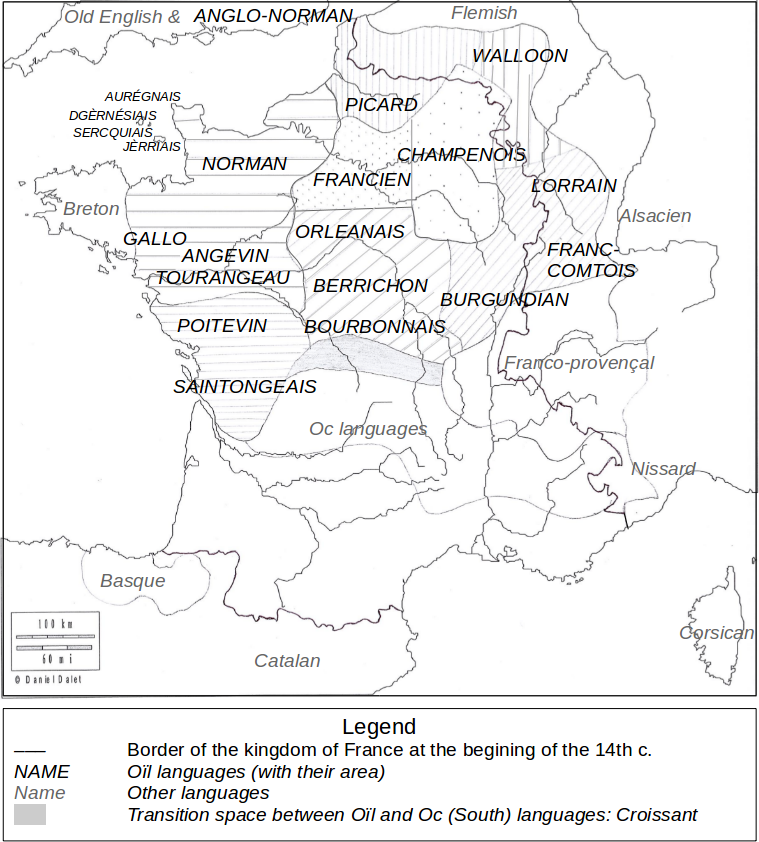
\includegraphics[scale=0.29]{static/media/mod_eval/bertrade/map-dialects2.png}
    \caption{Oïl languages}
    \label{fig:map-dialects}
\end{figure}

There are also many cases of syntactic ambiguity. For example, in the following quote from \emph{Lancelot},\footnote{In the edition from Pierre Kunstmann, from the online \textit{Base de français médiéval}: \url{http://catalog.bfm-corpus.org/CharretteKu}.} (verse ~5436),
both \enquote{la dame} and \enquote{Lancelot} could be the subject or the object of \enquote{Vit} and only the context enables the reader to understand that \enquote{la dame} is the subject.

    \digloss{Dolant et pansif Lancelot Vit la dame}
    {Mournful and meditative Lancelot saw the lady}
    {The lady saw that Lancelot was mournful and meditative.}

Word order is also relatively free within constituents. For example, a noun modifier can be on the left or on the right of its governor, and it is not necessarily preceded by a preposition. In contemporary French, it can only appear on the right, and it is found without a preposition only in some cases like named entities. Because of the general free word order and the absence of punctuation in our treebank, this adds up to the ambiguity of the analysis.

In each of the following examples from the SRCMF corpus, the noun following \emph{roi} (\enquote{king}) has a different analysis: head of \emph{roi}, modifier, argument of the same verb or a different one, with no explicit marking:

\begin{center}
    % beroul. modifieur à gauche.
    \begin{dependency}[theme=simple]
        \begin{deptext}[row 2/.style={font=\small}]
            \textit{Fus} \& \textit{tu} \& \textit{donc} \& \textit{pus} \& \textit{a} \& \textit{la} \& \textbf{\textit{roi}} \& \textit{cort} \\
            %VERB \& PRON \& ADV \& ADV \& ADP \& DET \& NOUN \& NOUN \\
            Were \& you \& then \& no more \& at \& the \& king \& court \\
        \end{deptext}
        \depedge{8}{7}{nmod}
        \depedge[edge start x offset=0.5em]{8}{6}{det}
        \depedge[edge start x offset=1em]{8}{5}{case}
    \end{dependency}

    \raggedright
    \enquote{Then were you not at the king's court anymore?} (\emph{Beroul Tristan})
\end{center}

\begin{center}
    % Graal. modifieur à droite.
    \begin{dependency}[theme=simple]
        \begin{deptext}[row 2/.style={font=\small}]
            \textit{la} \& \textit{fille} \& \textit{au} \& \textit{riche} \& \textbf{\textit{roi}} \& \textit{pescheor} \\
            the \& daughter \& of the \& rich \& king \& fisher \\
        \end{deptext}
        \depedge{5}{6}{flat}
    \end{dependency}

    \raggedright
    \enquote{the daughter of the rich Fisher King} (\emph{Queste del Saint Graal})
\end{center}

\begin{center}
    % Roland. arguments du même verbe.
    \begin{dependency}[theme=simple]
        \begin{deptext}[row 2/.style={font=\small}]
            \textit{De} \& \textit{Guenelun} \& \textit{atent} \& \textit{li} \& \textbf{\textit{reis}} \& \textit{nuveles} \\
            From \& Ganelon \& waits \& the \& king \& news \\
        \end{deptext}
        \depedge{3}{5}{nsubj}
        \depedge[edge start x offset=-0.5em]{3}{6}{obj}
    \end{dependency}

    \raggedright
    \enquote{The king waits for news from Ganelon.} (\emph{Chanson de Roland})
\end{center}

\begin{center}
    % Graal. arguments de verbes différents, et absence de ponctuation.
    \begin{dependency}[theme=simple]
        \begin{deptext}[row 2/.style={font=\small}]
            \textit{Biax} \& \textit{sire} \& \textit{fet} \& \textit{li} \& \textbf{\textit{rois}} \& \textit{escu} \& \textit{vos} \& \textit{envoiera} \& \textit{Diex} \\
            Dear \& Sir \& says \& the \& king \& shield \& you \& send-FUT \& God \\
        \end{deptext}
        \depedge{3}{5}{nsubj}
        \depedge{8}{6}{obj}
    \end{dependency}

    \raggedright
    \enquote{Dear Sir, says the king, God will send you a shield.} (\emph{Queste del Saint Graal})
\end{center}

Furthermore, overt subjects are not mandatory, and are often dropped in texts written in verse until the 12th century, after which the presence of subjects increases through time.
These phenomena are particularly prevalent in verse, where metric and rhyming constraints often lead to more contrived syntactic forms than in prose.

Another source of ambiguity is the variety of spellings, due to the lack of spelling standard. For example, the word \textit{moult} (transl. \textit{a lot (of), very}), emblematic of this period, is initially an adjective, and it is progressively grammaticalized, becoming an adverb. Several forms appear at the same time, some with a declension, some without, and the radical does not have a fixed spelling: \textit{molt(e)(s), molz, mult(e)(s), mul(t)z, mou(l)t}…

\subsection{Early Modern French}\label{def:early}

\begin{table*}[!htp]
    \centering\small
    \begin{tabular}{@{}p{0.3\linewidth}p{0.3\linewidth}p{0.3\linewidth}@{}}
        \toprule
        Source                                                                                                                                                                                                                                                                                               & Normalised & Translation \\
        \midrule
        Surquoy, SIRE, s’il plaiſt à voſtre Maieſté de ſe ſouuenir des miſeres de ſon Eſtat, dõt au moins ell’a tiré cét aduantage, qu’en vne grande ieuneſse ell’a acquis vne grande experi\~ece, elle verra que tous les mal-heurs de sõ bas âge ont pris leur commencement en ſemblables occaſions;       &
        \emph{Sur quoi, SIRE, s’il plaît à votre Majesté de se souvenir des misères de son état dont au moins elle a tiré cet avantage, qu’en une grande jeunesse elle a acquis une grande expérience, elle verra que tous les malheurs de son bas âge ont pris leur commencement en semblables occasions~;} &
        \textcolor{gray}{``Whereupon, SIR, if it pleases your Majesty to remember the miseries of her state, from which at least she has derived this advantage, that in great youth she has acquired great experience, she will see that all the misfortunes of her early life took their beginning on similar occasions;''}           \\
        \bottomrule
    \end{tabular}
    \caption{\label{tab:norm_examples}Example of normalisation taken from the \emph{Lettres} of \protect\newcite{balzac-1624-lettres}.}
\end{table*}

We loosely define Early Modern French as a state of language following Middle French in 1500---following here the \emph{terminus ad quem} used by the \emph{Dictionnaire de Moyen Français} \cite{martin-2020-dictionnaire}---and ending with the French Revolution in 1789. It therefore encompasses three centuries (16\textsuperscript{th}, 17\textsuperscript{th} and 18\textsuperscript{th}\,c.), or two linguistic periods: the \emph{français préclassique} or ``preclassical French'', 1500--1630 and the \emph{français classique} or ``classical French'', 1630--1689; both periodisations are currently used in French linguistics (\emph{e.g.}~by \newcite{vachon-2010-changement} and \newcite{amatuzzi-etal-2019-ameliorer}).

A typical example of Early Modern French, taken from ~\newcite{balzac-1624-lettres}, is given in Table~\ref{tab:norm_examples}. We note here the presence of several phenomena that have now disappeared in contemporary French, such as the presence of abbreviations (\emph{dõt}$\to$\emph{dont}), the long \emph{s} (\emph{ſ}, see\,\emph{miſeres}), the use of \emph{v} instead of \emph{u} (\emph{vne} for \emph{une}), the conservation of etymological letters (\emph{voſtre}$<$Latin~\emph{vŏster} rather than \emph{votre}) and calligraphic letters (\emph{-y} in \emph{Surquoy}), the absence of welding  (\emph{\mbox{mal-heurs}} and not \emph{malheurs}) and the opposite (\emph{Surquoy} and not \emph{Sur quoi}).

For NLP tasks, which process raw sequences, such differences with respect to contemporary French are not trivial, and they prevent the processing of historical texts with tools trained on recent sources.

\section{Outline}

